\chapter{Requisits del sistema}
\usetikzlibrary{positioning, shadows}
\label{chap:requisits}

Abans d'iniciar el desenvolupament de l'aplicació NUMEN, s'ha dut a terme una anàlisi detallada de requisits, seguint una metodologia rigorosa per garantir l'èxit del projecte. Aquesta fase ha estat clau per identificar les funcionalitats necessàries, establir les característiques tècniques que ha de complir el sistema i definir-ne l'abast, assegurant que la solució final satisfaci les necessitats de l'usuari expert, tant en l'àmbit del càlcul numerològic complex com en la interpretació assistida per Intel·ligència Artificial.

Els requisits s'han classificat en funcionals, no funcionals i de domini, codificant-los per facilitar-ne la traçabilitat i assignant-los una prioritat (alta, mitjana o baixa) en funció de la seva importància per al correcte funcionament del sistema. A més, per facilitar l'anàlisi de dependències i la planificació del desenvolupament, s'han agrupat en blocs lògics.

Tot seguit, es presenta un glossari amb els termes principals utilitzats al llarg d'aquest capítol, per garantir-ne la claredat i coherència terminològica.

\section{Glossari de Termes}

\begin{description}
    \item[App Web / Escriptori] Aplicació híbrida desenvolupada en Flutter \cite{flutter_web}. Funciona principalment com a aplicació web accessible des de qualsevol navegador, però conserva la capacitat de compilar-se com a executables d'escriptori (Windows) per a ús \textit{offline} si és necessari.

    \item[Sistema] El programari NUMEN en si mateix, que executa processos automàtics, càlculs i interaccions sense intervenció humana directa en aquell instant.
    \item[Figura Espiritual] Representació gràfica dinàmica de l'Home de Vitruvi, construïda visualment via manipulació de vectors SVG en funció de les dades de l'usuari.
    \item[Nombres Kàrmics] Nombres buits (valor buit = 0) que indiquen lliçons pendents.
    \item[Prompt] Instrucció textual estructurada que s'envia a l'IA \cite{gemini_model, openai_prompt_engineering, google_prompt_engineering}.
\end{description}

\section{Esquema del Sistema}

El sistema NUMEN compta amb tres actors principals, cadascun amb un rol ben definit:

\begin{itemize}
    \item \textbf{Administrador (Tècnic):} Perfil tècnic encarregat del manteniment del sistema, resolució d'incidències i actualització dels \textit{prompts} o la infraestructura.
    \item \textbf{Usuari (Professional):} Numeròleg/a que utilitza la part privada de l'aplicació per generar informes, gestionar l'historial i compartir resultats amb els clients finals.
    \item \textbf{Visitant Públic:} Usuari anònim que accedeix a la part pública per consultar informació, veure testimonis o provar la demo gratuïta.
    \item \textbf{Client Final:} Persona interessada que rep un informe complet (PDF o enllaç) o contracta els serveis professionals.
\end{itemize}

La Figura \ref{fig:esquema_sistema} il·lustra les interaccions d'alt nivell entre aquests actors i els components del sistema.

\begin{figure}[h]
    \centering
    \begin{tikzpicture}[node distance=2.5cm, auto,
        actor/.style={circle, draw, minimum size=1cm, inner sep=0pt, fill=gray!10},
        block/.style={rectangle, draw, rounded corners, minimum width=2.5cm, minimum height=1.5cm, fill=blue!10, align=center},
        cloudNode/.style={cloud, draw, cloud puffs=10, cloud puff arc=120, aspect=2, minimum width=3cm, fill=green!10, align=center},
        line/.style={draw, -latex', thick}]

        % Nodes
        % Nodes
        \node [actor] (client) {Client};
        \node [actor, above of=client, node distance=2cm] (visitant) {Visitant};
        
        \node [block, right of=visitant, node distance=5cm, yshift=-1.25cm] (app_public) {App Pública\\(Web + Demo)};
        \node [block, below of=app_public, node distance=5cm] (app_private) {App Privada\\(Gestió + Càlcul)};
        
        \node [actor, left of=app_private, node distance=7cm] (admin) {Usuari};
        
        \node [cloudNode, right of=app_private, node distance=5cm] (db) {Base de Dades\\(FireBase \cite{firebase_platform})};
        \node [block, above of=db, node distance=5cm] (ai) {Servei IA\\(API)};

        % Edges Public to/from Actors
        \path [line] (visitant) -- node[above, sloped] {Visita/Demo} (app_public);
        \path [line] (client) -- node[above, sloped] {Feedback} (app_public);
        
        % Cross-Apps diagonals (Left side)
        % Public -> Admin (WhatsApp)
        \path [line] (app_public) -- node[pos=0.7, above, sloped] {WhatsApp} (admin); 
        % Private -> Client (Link)
        \path [line] (app_private) -- node[pos=0.2, above, sloped] {Genera Link} (client);

        % Edges Private
        \path [line] (admin) -- node[above] {Login/Full Access} (app_private);
        \path [line] (app_private) -- node[above] {CRUD} (db);
        
        % Cross-Apps diagonals (Right side)
        % Private -> AI (Prompt)
        \path [line] (app_private) -- node[pos=0.3, below, sloped] {Prompt} (ai);
        % Public -> DB (Read)
        \path [line] (app_public) -- node[pos=0.3, above, sloped] {Testimonis} (db);
        
        % AI Back
        \path [line] (ai) -- node[pos=0.2, below, sloped] {Interpretació} (app_private);

    \end{tikzpicture}
    \caption{Esquema d'alt nivell del sistema NUMEN (Arquitectura Híbrida).}
    \label{fig:esquema_sistema}
\end{figure}

\section{Requeriments del Sistema}

\subsection{Requeriments Funcionals}

\begin{table}[H]
    \centering
    \begin{tabular}{|l|l|l|p{8cm}|}
    \hline
    \textbf{ID} & \textbf{Prioritat} & \textbf{Actor} & \textbf{Descripció} \\ \hline
    RF1 & Alta & Usuari & El sistema ha de permetre introduir la data de naixement i nom complet. \\ \hline
    RF2 & Alta & Sistema & Execució automàtica dels algorismes de càlcul (Gematria, Cicles, NL). \\ \hline
    RF3 & Alta & Sistema & Visualització de resultats en graelles i llistes. \\ \hline
    RF4 & Alta & Sistema & Generació dinàmica de l'Home de Vitruvi (SVG) segons dades. \\ \hline
    RF5 & Alta & Sistema & Detecció i marcatge visual de Karmes i Nombres Mestres. \\ \hline
    RF6 & Alta & Usuari & L'usuari ha de poder sol·licitar una interpretació a la IA. \\ \hline
    RF7 & Alta & Sistema & Mostratge de la interpretació en format text natural estructurat. \\ \hline
    RF8 & Mitja & Usuari & L'usuari ha de veure l'opció de valorar la resposta (estrelles) i text. \\ \hline
    RF9 & Alta & Sistema & Emmagatzematge persistent de consultes i feedback (Firestore). \\ \hline
    RF10 & Alta & Sistema & Generació d'informe en \textbf{PDF Natiu} (Vectorial) descarregable. \\ \hline
    RF11 & Mitja & Usuari & Gestió interna de l'aplicació (manteniment de prompts). \\ \hline
    RF12 & Mitja & Sistema & Configuració de paràmetres globals (idioma, etc.). \\ \hline
    RF13 & Alta & Sistema & Generació d'un ``Enllaç Compartit'' amb caducitat de 24h. \\ \hline
    RF14 & Alta & Sistema & Adaptació de la interfície a dispositius mòbils (\textbf{Responsive Design}). \\ \hline
    RF15 & Alta & Sistema & Sistema d'Autenticació (Login) per restringir l'accés a l'usuari professional. \\ \hline
    RF16 & Mitja & Client & Portal públic amb contingut educatiu, demo (Tastet) i \textbf{contacte via WhatsApp}. \\ \hline
    RF17 & Alta & Usuari & Visualització, filtratge i gestió de l'historial d'estudis (Base de Dades). \\ \hline
    \end{tabular}

    \caption{Requisits funcionals del sistema.}
    \label{tab:req_funcionals}
\end{table}

\subsection{Matriu de dependències entre requisits funcionals}

\begin{table}[H]
    \centering
    \resizebox{\textwidth}{!}{%
    \begin{tabular}{|l|c|c|c|c|c|c|c|c|c|c|c|c|c|c|c|c|c|}
    \hline
         & \textbf{RF1} & \textbf{RF2} & \textbf{RF3} & \textbf{RF4} & \textbf{RF5} & \textbf{RF6} & \textbf{RF7} & \textbf{RF8} & \textbf{RF9} & \textbf{RF10} & \textbf{RF11} & \textbf{RF12} & \textbf{RF13} & \textbf{RF14} & \textbf{RF15} & \textbf{RF16} & \textbf{RF17} \\ \hline
    \textbf{RF1} & & X & & & & & & & & & & & & & & & \\ \hline
    \textbf{RF2} & & & X & X & X & X & & & & X & & & & & & X & \\ \hline
    \textbf{RF3} & & & & & & & & & & X & & & X & & & & \\ \hline
    \textbf{RF4} & & & & & & & & & & X & & & & & & & \\ \hline
    \textbf{RF5} & & & & & & & & & & X & & & & & & & \\ \hline
    \textbf{RF6} & & & & & & & X & & X & & & & & & & & \\ \hline
    \textbf{RF7} & & & & & & & & X & X & X & & & X & & & & \\ \hline
    \textbf{RF8} & & & & & & & & & X & & & & & & & & \\ \hline
    \textbf{RF9} & & & & & & & & & & & X & & & & & & X \\ \hline
    \textbf{RF10}& & & & & & & & & & & & & X & & & & \\ \hline
    \textbf{RF11}& & & & & & & & & & & & X & & & & & \\ \hline
    \textbf{RF12}& & & & & & & & & & & & & & & & & \\ \hline
    \textbf{RF13}& & & & & & & & & & & & & & & & & \\ \hline
    \textbf{RF14}& & & & & & & & & & & & & & & & & \\ \hline
    \textbf{RF15}& & & & & & & & & & & & & & & & & X \\ \hline
    \textbf{RF16}& & & & & & & & & & & & & & & & & \\ \hline
    \textbf{RF17}& & & & & & & & & & & & & & & & & \\ \hline
    \end{tabular}%
    }
    \caption{Matriu de dependències entre requisits funcionals.}
    \label{tab:dependencies_func}
\end{table}

\subsection{Requeriments No Funcionals}

\begin{table}[H]
    \centering
    \begin{tabular}{|l|l|p{5cm}|p{5cm}|}
    \hline
    \textbf{ID} & \textbf{Prioritat} & \textbf{Descripció} & \textbf{Verificació} \\ \hline
    RNF1 & Alta & Usabilitat intuïtiva (Mobile First). & Test d'usuari sense formació prèvia. \\ \hline
    RNF2 & Mitja & Latència IA < 10s. & Mesura en xarxa 4G/Fibra. \\ \hline
    RNF3 & Alta & Compatibilitat Web i Escriptori (Windows). & Execució en Chrome, Edge i .exe natiu. \\ \hline
    RNF4 & Alta & Seguretat de les dades (Regles Firestore). & Intent d'accés no autoritzat bloquejat. \\ \hline
    RNF5 & Alta & Qualitat d'impressió professional. & PDF vectorial escalable sense pixelat. \\ \hline
    \end{tabular}
    \caption{Requisits no funcionals del sistema.}
    \label{tab:req_nofuncionals}
\end{table}

\subsection{Requeriments del Domini}

\begin{table}[H]
    \centering
    \begin{tabular}{|l|l|p{10cm}|}
    \hline
    \textbf{ID} & \textbf{Prioritat} & \textbf{Descripció} \\ \hline
    RD1 & Alta & Càlculs estrictes segons Mètode Coquatrix. \\ \hline
    RD2 & Alta & To de la IA: Empàtic, constructiu i respectuós. \\ \hline
    RD3 & Mitja & Privacitat: Anonimització de dades sensibles en logs. \\ \hline
    RD4 & Alta & Tractament correcte de Nombres Mestres (11, 22, 33). \\ \hline
    RD5 & Alta & La Figura Espiritual ha de respectar la geometria sagrada definida en el marc teòric. \\ \hline
    \end{tabular}
    \caption{Requisits del domini.}
    \label{tab:req_domini}
\end{table}

\section{Matriu de dependències entre tots els requisits}

\begin{table}[H]
    \centering
    \resizebox{\textwidth}{!}{%
    \begin{tabular}{|l|c|c|c|c|c|c|c|c|c|c|c|c|c|c|c|c|c|c|c|c|c|c|c|c|c|c|c|}
    \hline
         & \textbf{\rotatebox{90}{RF1}} & \textbf{\rotatebox{90}{RF2}} & \textbf{\rotatebox{90}{RF3}} & \textbf{\rotatebox{90}{RF4}} & \textbf{\rotatebox{90}{RF5}} & \textbf{\rotatebox{90}{RF6}} & \textbf{\rotatebox{90}{RF7}} & \textbf{\rotatebox{90}{RF8}} & \textbf{\rotatebox{90}{RF9}} & \textbf{\rotatebox{90}{RF10}} & \textbf{\rotatebox{90}{RF11}} & \textbf{\rotatebox{90}{RF12}} & \textbf{\rotatebox{90}{RF13}} & \textbf{\rotatebox{90}{RF14}} & \textbf{\rotatebox{90}{RF15}} & \textbf{\rotatebox{90}{RF16}} & \textbf{\rotatebox{90}{RF17}} & \textbf{\rotatebox{90}{RNF1}} & \textbf{\rotatebox{90}{RNF2}} & \textbf{\rotatebox{90}{RNF3}} & \textbf{\rotatebox{90}{RNF4}} & \textbf{\rotatebox{90}{RNF5}} & \textbf{\rotatebox{90}{RD1}} & \textbf{\rotatebox{90}{RD2}} & \textbf{\rotatebox{90}{RD3}} & \textbf{\rotatebox{90}{RD4}} & \textbf{\rotatebox{90}{RD5}} \\ \hline
    \textbf{RF1} & & X & & & & & & & & & & & & & & & & & & & & & & & & & \\ \hline
    \textbf{RF2} & & & X & X & X & X & & & & X & & & & & & X & & & & & & X & & X & & X & \\ \hline
    \textbf{RF3} & & & & & & & & & & X & & & X & & & & & X & & & & & & & & & \\ \hline
    \textbf{RF4} & & & & & & & & & & X & & & & & & & & & & & & & & & & & X \\ \hline
    \textbf{RF5} & & & & & & & & & & X & & & & & & & & & & & & & & & & & \\ \hline
    \textbf{RF6} & & & & & & & X & & X & & & & & & & & & & X & & & & & & & & \\ \hline
    \textbf{RF7} & & & & & & & & X & X & X & & & X & & & & & X & & & & & & X & & & \\ \hline
    \textbf{RF8} & & & & & & & & & X & & & & & & & & & & & & & & & & & & \\ \hline
    \textbf{RF9} & & & & & & & & & & & X & & & & & & X & & & X & & & X & & & &\\ \hline
    \textbf{RF10}& & & & & & & & & & & & & X & & & & & & & & X & & & & & & \\ \hline
    \textbf{RF11}& & & & & & & & & & & & X & & & & & & & & X & & & & X & & & \\ \hline
    \textbf{RF12}& & & & & & & & & & & & & & & & & & & & & X & & & & & & \\ \hline
    \textbf{RF13}& & & & & & & & & & & & & & & & & & & & & & & & & & & \\ \hline
    \textbf{RF14}& & & & & & & & & & & & & & & X & & X & & & & & & & & & & \\ \hline
    \textbf{RF15}& & & & & & & & & & & & & & & & & X & & & & X & & & & & & \\ \hline
    \textbf{RF16}& & & & & & & & & & & & & & & & & & X & & & & & & & & & \\ \hline
    \textbf{RF17}& & & & & & & & & X & & & & & & & & & & & & & & & & & & \\ \hline
    \end{tabular}%
    }
    \caption{Matriu de dependències global.}
    \label{tab:dependencies_global}
\end{table}



\section{Relació amb la Planificació (Mapatge de Requisits)}

La Figura \ref{fig:mapa_requisits} il·lustra com els requisits s'implementen a través dels Paquets de Treball (PT) definits al Capítol 4.

\begin{figure}[H]
    \centering
    \resizebox{1.1\textwidth}{!}{%
    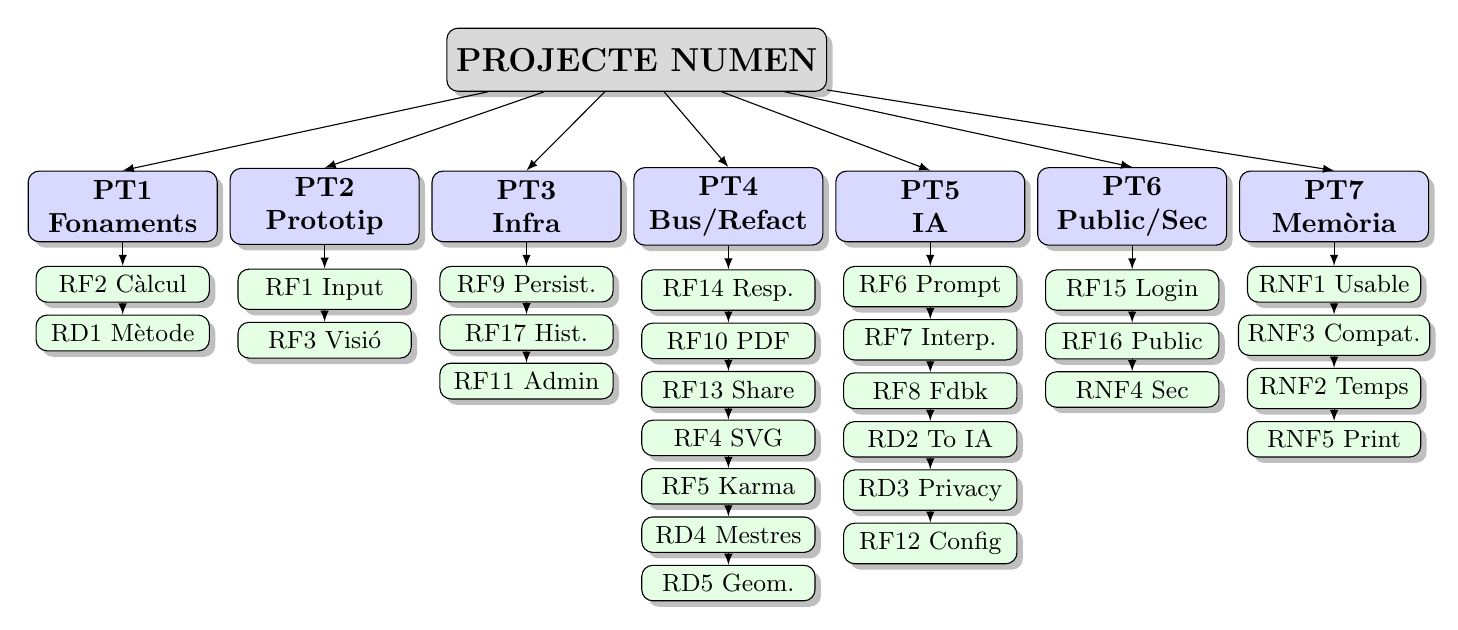
\begin{tikzpicture}[
        node distance=0.5cm and 0.4cm,
        every node/.style={draw, rounded corners, align=center, font=\scriptsize, fill=white, drop shadow},
        root/.style={fill=gray!30, font=\large\bfseries, minimum width=3cm, minimum height=0.8cm},
        pt/.style={fill=blue!15, font=\bfseries, minimum width=2.4cm, minimum height=0.7cm},
        req/.style={fill=green!10, font=\small, minimum width=2.2cm, minimum height=0.45cm},
        link/.style={-latex, thin}
    ]

    % Root
    \node[root] (root) {PROJECTE NUMEN};

    % Level 2: PTs (Centered flat structure)
    % Center split: PT3 and PT4 are in the middle
    \node[pt, below=1cm of root, xshift=-1.4cm] (pt3) {PT3\\Infra};
    \node[pt, right=0.15cm of pt3] (pt4) {PT4\\Bus/Refact};
    
    % Left wing
    \node[pt, left=0.15cm of pt3] (pt2) {PT2\\Prototip};
    \node[pt, left=0.15cm of pt2] (pt1) {PT1\\Fonaments};

    % Right wing
    \node[pt, right=0.15cm of pt4] (pt5) {PT5\\IA};
    \node[pt, right=0.15cm of pt5] (pt6) {PT6\\Public/Sec};
    \node[pt, right=0.15cm of pt6] (pt7) {PT7\\Memòria};

    % Links Root -> PTs
    \draw[link] (root) -- (pt1.north);
    \draw[link] (root) -- (pt2.north);
    \draw[link] (root) -- (pt3.north);
    \draw[link] (root) -- (pt4.north);
    \draw[link] (root) -- (pt5.north);
    \draw[link] (root) -- (pt6.north);
    \draw[link] (root) -- (pt7.north);

    % Level 3: Requirements (Vertical Stacks)
    
    % PT1 (Fonaments) -> RF2, RD1
    \node[req, below=0.3cm of pt1] (rf2) {RF2 Càlcul};
    \node[req, below=0.15cm of rf2] (rd1) {RD1 Mètode};
    \draw[link] (pt1) -- (rf2);
    \draw[link] (rf2) -- (rd1);

    % PT2 (Prototip) -> RF1, RF3
    \node[req, below=0.3cm of pt2] (rf1) {RF1 Input};
    \node[req, below=0.15cm of rf1] (rf3) {RF3 Visió};
    \draw[link] (pt2) -- (rf1);
    \draw[link] (rf1) -- (rf3);

    % PT3 (Infra) -> RF9(DB), RF17(History), RF11(Admin)
    \node[req, below=0.3cm of pt3] (rf9) {RF9 Persist.};
    \node[req, below=0.15cm of rf9] (rf17) {RF17 Hist.};
    \node[req, below=0.15cm of rf17] (rf11) {RF11 Admin};
    \draw[link] (pt3) -- (rf9);
    \draw[link] (rf9) -- (rf17);
    \draw[link] (rf17) -- (rf11);

    % PT4 (Refactor) -> RF14, RF10, RF13, RF4, RF5, RD4, RD5
    \node[req, below=0.3cm of pt4] (rf14) {RF14 Resp.};
    \node[req, below=0.15cm of rf14] (rf10) {RF10 PDF};
    \node[req, below=0.15cm of rf10] (rf13) {RF13 Share};
    \node[req, below=0.15cm of rf13] (rf4) {RF4 SVG};
    \node[req, below=0.15cm of rf4] (rf5) {RF5 Karma};
    \node[req, below=0.15cm of rf5] (rd4) {RD4 Mestres};
    \node[req, below=0.15cm of rd4] (rd5) {RD5 Geom.};
    \draw[link] (pt4) -- (rf14);
    \draw[link] (rf14) -- (rf10);
    \draw[link] (rf10) -- (rf13);
    \draw[link] (rf13) -- (rf4);
    \draw[link] (rf4) -- (rf5);
    \draw[link] (rf5) -- (rd4);
    \draw[link] (rd4) -- (rd5);

    % PT5 (IA) -> RF6, RF7, RF8, RD2, RD3, RF12
    \node[req, below=0.3cm of pt5] (rf6) {RF6 Prompt};
    \node[req, below=0.15cm of rf6] (rf7) {RF7 Interp.};
    \node[req, below=0.15cm of rf7] (rf8) {RF8 Fdbk};
    \node[req, below=0.15cm of rf8] (rd2) {RD2 To IA};
    \node[req, below=0.15cm of rd2] (rd3) {RD3 Privacy};
    \node[req, below=0.15cm of rd3] (rf12) {RF12 Config};
    \draw[link] (pt5) -- (rf6);
    \draw[link] (rf6) -- (rf7);
    \draw[link] (rf7) -- (rf8);
    \draw[link] (rf8) -- (rd2);
    \draw[link] (rd2) -- (rd3);
    \draw[link] (rd3) -- (rf12);

    % PT6 (Public/Sec) -> RF15, RF16, RNF4
    \node[req, below=0.3cm of pt6] (rf15) {RF15 Login};
    \node[req, below=0.15cm of rf15] (rf16) {RF16 Public};
    \node[req, below=0.15cm of rf16] (rnf4) {RNF4 Sec};
    \draw[link] (pt6) -- (rf15);
    \draw[link] (rf15) -- (rf16);
    \draw[link] (rf16) -- (rnf4);
    
    % PT7 (Memòria/Validació) -> RNF1, RNF2, RNF3, RNF5
    \node[req, below=0.3cm of pt7] (rnf1) {RNF1 Usable};
    \node[req, below=0.15cm of rnf1] (rnf3) {RNF3 Compat.};
    \node[req, below=0.15cm of rnf3] (rnf2) {RNF2 Temps};
    \node[req, below=0.15cm of rnf2] (rnf5) {RNF5 Print};
    \draw[link] (pt7) -- (rnf1);
    \draw[link] (rnf1) -- (rnf3);
    \draw[link] (rnf3) -- (rnf2);
    \draw[link] (rnf2) -- (rnf5);

    \end{tikzpicture}%
    }
    \caption{Traçabilitat entre Paquets de Treball i Requisits.}
    \label{fig:mapa_requisits}
\end{figure}
